\documentclass{article}

\IfFileExists{neurips_2024.sty}{%
  \usepackage[final]{neurips_2024}
}{%
  \usepackage[letterpaper,margin=1in]{geometry}
  \usepackage{times}
}

\usepackage[T1]{fontenc}
\usepackage[utf8]{inputenc}
\usepackage{microtype}
\usepackage{graphicx}
\usepackage{subcaption}
\usepackage{booktabs}
\usepackage{amsmath}
\usepackage{xcolor}
\usepackage{hyperref}
\usepackage{enumitem}
\usepackage{float}

% Relax float placement constraints so figures stay near their text
\renewcommand{\topfraction}{0.9}
\renewcommand{\bottomfraction}{0.8}
\renewcommand{\textfraction}{0.05}
\renewcommand{\floatpagefraction}{0.8}
\setcounter{topnumber}{9}
\setcounter{bottomnumber}{9}
\setcounter{totalnumber}{9}

\hypersetup{
  colorlinks=true,
  linkcolor=black,
  citecolor=black,
  urlcolor=blue
}

\setlist[itemize]{leftmargin=1.2em,itemsep=2pt,topsep=3pt}
\setlist[enumerate]{leftmargin=1.4em,itemsep=2pt,topsep=3pt}

\title{Memory-Efficient Quantized GPT-2 Training in Raw C/CUDA}

\author{%
  Pragnay Mandavilli \\
  Raju Kanumuri \\
  Ayush Yadav \\
  Efficient AI Course Project
}

\begin{document}

\maketitle

\begin{abstract}
Training GPT-style language models is memory intensive because parameters, gradients,
optimizer moments, master weights, and saved activations must remain resident on the GPU.
This project modifies Karpathy's \texttt{llm.c} GPT-2 training implementation into a
quantization-aware training system written in pure C/CUDA. The system stores the four large
transformer projection matrices in low precision (\texttt{INT8}, \texttt{FP8 E4M3}, or
grouped \texttt{INT4}), dequantizes each layer's weights on demand for cuBLASLt matmuls,
updates parameters with AdamW, and re-quantizes the trained weights after every optimizer
step. It also compresses AdamW optimizer states using COAT-style per-group scaling and
dynamic range expansion for \texttt{FP8}, \texttt{INT8}, and \texttt{INT4} moment storage.
The experiments show a clear progression: \texttt{FP8} and \texttt{INT8} weight
quantization preserve training-loss behavior, \texttt{INT4} requires smaller quantization
groups, optimizer-state quantization remains stable across tested precisions, naive
grid-based attention activation quantization diverges, and COAT-style activation grouping restores
stable training. The combined configuration reduces measured memory from 3.81 GiB to
2.67 GiB, a 30\% reduction.
\end{abstract}

\section{Introduction}

Large language models are limited not only by arithmetic throughput but also by GPU memory.
Even for GPT-2 124M, training with mixed precision stores several copies of model-related
state: the forward weights in \texttt{floatX} (\texttt{BF16} or \texttt{FP32} depending on
the build), gradients in \texttt{floatX}, AdamW's first and second moments in \texttt{FP32},
and a separate \texttt{FP32} master copy of the weights. Larger contexts add another major
term through saved activations. The consequence is that many memory-saving ideas must target
training state, not only inference weights.

This project starts from \texttt{llm.c}, a pure C/CUDA implementation of GPT-2/GPT-3-style
pretraining. The codebase is useful for an Efficient AI project because memory layout is
explicit: parameters, gradients, activations, and optimizer state are each allocated as large
contiguous buffers and then pointed into by typed tensor views. That makes it possible to
change storage formats without hiding behind framework-level abstractions.

The goal of the project is to move from ordinary mixed-precision training toward
quantization-aware training. In the implementation, \texttt{PTQ} in function and flag names
is historically inherited, but the training behavior is closer to weight-only QAT. The
forward and backward passes repeatedly use dequantized versions of quantized weights,
gradients are accumulated with respect to those dequantized weights, the optimizer updates
the stored \texttt{floatX} parameters, and the result is quantized again before the next
step. This is the standard fake-quantization pattern with an implicit straight-through
estimator, implemented manually in CUDA.

\section{Individual Contribution}

This project was completed by Pragnay Mandavilli, Raju Kanumuri, and Ayush Yadav. The
individual contributions were:

\begin{itemize}
  \item \textbf{Ayush Yadav} worked on weight quantization, including low-precision storage
  for the large transformer projection matrices and group-size experiments for
  \texttt{INT4} weight quantization.
  \item \textbf{Raju Kanumuri} worked on optimizer-state quantization, including COAT-style
  low-precision AdamW moment storage with per-group scales and dynamic range expansion.
  \item \textbf{Pragnay Mandavilli} worked on experiments and activation quantization,
  including training-loss comparisons, memory-breakdown analysis, and activation grouping
  experiments.
\end{itemize}

Together, these contributions form an end-to-end low-precision training pipeline:
quantized model weights, quantized optimizer states, activation-quantization experiments,
and memory/loss evaluation.

\section{Problem Description}

The baseline training memory cost for a parameter that participates in AdamW is larger than
the model weight itself. In a BF16 training build with master weights, one parameter can
require approximately two bytes for the model weight, two bytes for the gradient, four bytes
for the master copy, four bytes for the first moment $m$, and four bytes for the second
moment $v$. The exact accounting depends on sharding and activation recomputation, but the
optimizer state and master copy dominate the memory cost.

The project asks whether GPT-2 training can keep the optimization behavior close to the
baseline while storing major tensors at 8-bit or 4-bit precision. The work is deliberately
staged from lowest risk to highest risk:

\begin{enumerate}
  \item Quantize weights while keeping the forward/backward numerics stable. This is the
  easiest entry point because weights are relatively stationary and roughly symmetric.
  \item Quantize optimizer states without destroying AdamW's moment estimates. This saves
  substantial memory, but the moment tensors have narrow, time-varying distributions.
  \item Quantize saved activations without causing gradient blow-up in attention or MLP
  layers. This is the hardest stage because activations are input-dependent and attention is
  numerically sensitive.
\end{enumerate}

The final system addresses all three stages experimentally. Weight and optimizer-state
quantization provide the stable core of the method, while activation quantization is treated
as the numerically sensitive stage whose grouping choice determines whether training remains
stable.

\section{Related Work}

Classical QAT inserts fake-quantization operations during training so that the model learns
under the rounding error it will see at inference time. Jacob et al.~\cite{jacob2017quantization}
introduced an integer-only inference pipeline with a training procedure that preserves
accuracy after quantization, establishing the basic idea of simulating low-precision
arithmetic while maintaining higher-precision learning state.

For large language models, post-training quantization work shows why Transformers need
special care. \texttt{LLM.int8()}~\cite{dettmers2022llmint8} isolates outlier feature
dimensions and handles them in higher precision while quantizing most matrix multiplication
work to 8-bit. SmoothQuant~\cite{xiao2022smoothquant} observes that weights are easier to
quantize than activations and migrates activation outlier difficulty into weights through an
offline equivalent transformation, enabling practical W8A8 inference. Both papers motivate
this project's decision to begin with weights and to treat activation quantization as a
harder later stage.

COAT~\cite{xi2024coat} is the most direct match for the optimizer-state part of this
project. COAT targets FP8 training memory by compressing optimizer states and activations,
using dynamic range expansion for optimizer moments and mixed-granularity activation
quantization. Our implementation adopts the same core idea for optimizer state: moments are
dequantized to \texttt{FP32}, AdamW math runs in \texttt{FP32}, and the updated moments are
expanded, scaled, and quantized back to low precision per group.

\section{Method}

Figure~\ref{fig:qat-arch} gives an overview of the full quantized training pipeline. The
following subsections describe each component in detail.

\begin{figure}[H]
  \centering
  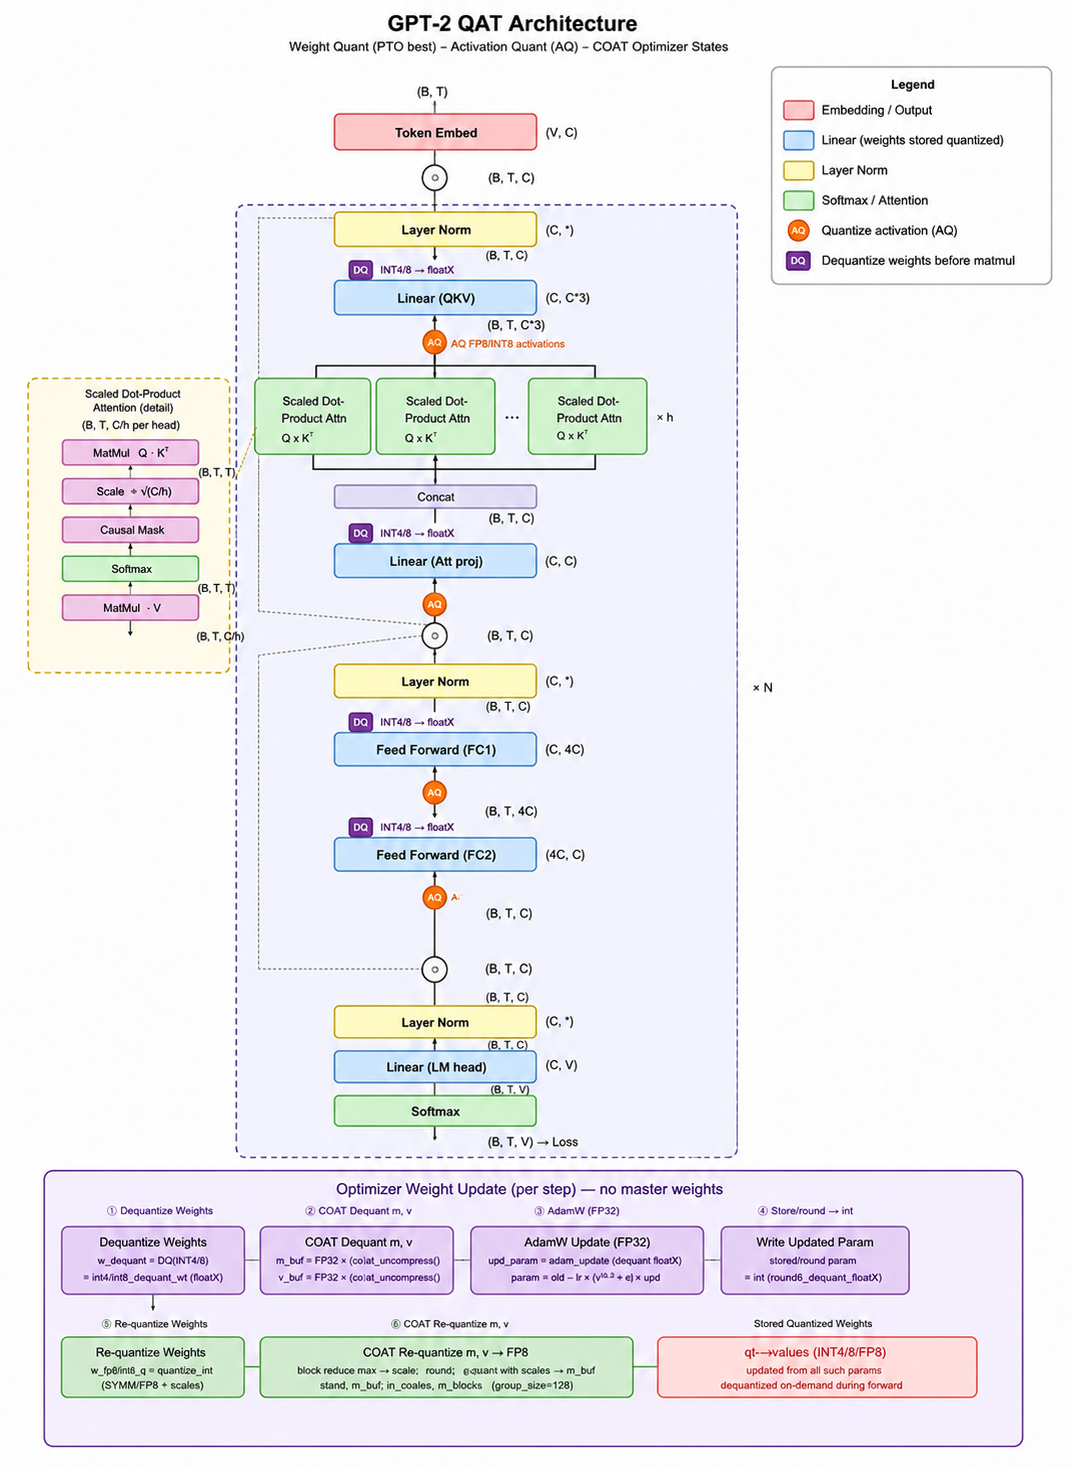
\includegraphics[width=0.92\linewidth]{figures/architecture_after_QAT.png}
  \caption{GPT-2 QAT architecture overview. Green blocks indicate weight quantization
  (QAT/PTQ), orange markers indicate activation quantization, and the table at the bottom
  summarises the COAT-style optimizer-state quantization applied to AdamW moments.}
  \label{fig:qat-arch}
\end{figure}

\subsection{Base Model and Numerical Conventions}

The base model is a GPT-2 decoder-only Transformer with token and positional embeddings,
repeated pre-norm attention/MLP blocks, a final layer norm, and a weight-tied language-model
head. Figure~\ref{fig:base-arch} shows the unmodified architecture. The project preserves
the original \texttt{llm.c} mixed-precision convention. Forward and backward tensors use
\texttt{floatX}, which is selected at compile time as \texttt{FP32} or \texttt{BF16};
sensitive statistics such as layer-norm means, inverse standard deviations, and loss buffers
remain \texttt{FP32}; and AdamW math promotes gradients to \texttt{FP32}.

\begin{figure}[H]
  \centering
  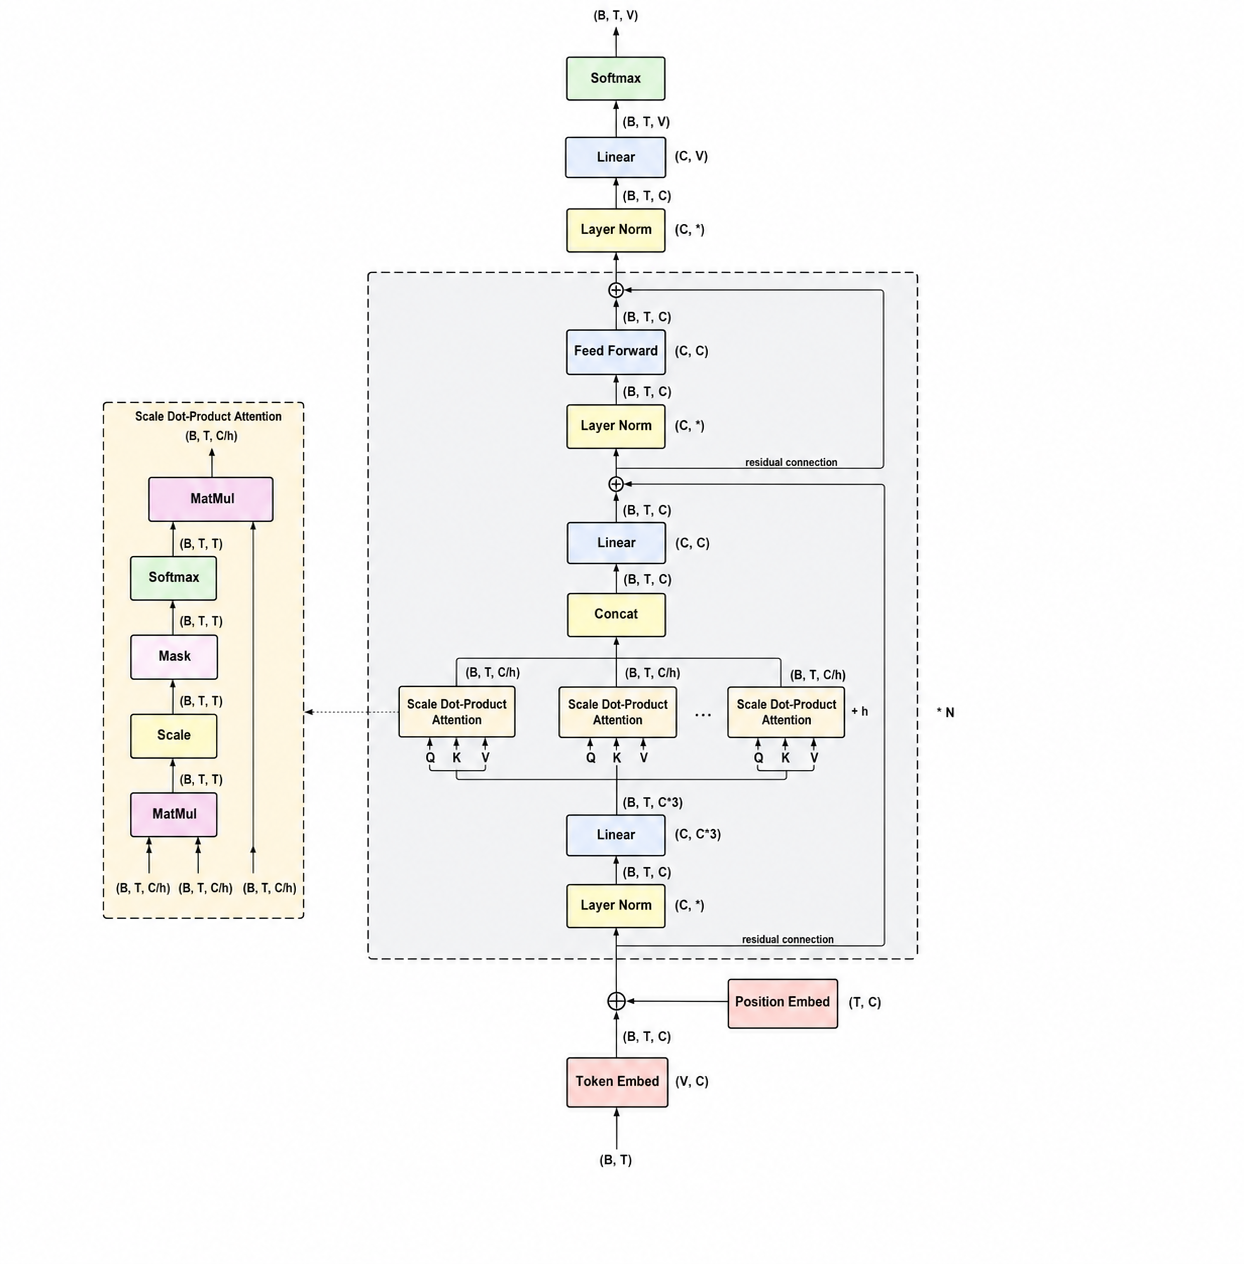
\includegraphics[width=0.52\linewidth]{figures/initial_architecture.png}
  \caption{Baseline GPT-2 decoder-only architecture before any quantization modifications.}
  \label{fig:base-arch}
\end{figure}

The important engineering invariant is that quantized storage is not used directly as GEMM
input. The code dequantizes a layer slice into \texttt{scratch\_dequant}, then calls the
existing cuBLASLt matmul path. This means the current implementation is a memory-saving and
training-noise experiment, not a true INT8 or FP8 tensor-core GEMM implementation.

\subsection{Weight Quantization: First Make the Model See Low-Precision Weights}

The central type is \texttt{QuantizedTensor}, which stores a byte payload
\texttt{qvalues}, floating-point \texttt{scales}, shape metadata, and a
\texttt{group\_size}. The precision enum supports \texttt{INT8}, \texttt{FP8}, and
\texttt{INT4}. \texttt{INT8} uses a signed symmetric range $[-127,127]$, \texttt{INT4}
uses $[-7,7]$, and \texttt{FP8} uses CUDA's native \texttt{\_\_nv\_fp8\_e4m3}
conversion with maximum finite magnitude 448.

For a row or group of weights, the quantizer computes
\[
  s = \frac{\max_i |w_i|}{Q_{\max}}
\]
and writes
\[
  q_i = \operatorname{round}\left(\operatorname{clip}(w_i/s, -Q_{\max}, Q_{\max})\right).
\]
For \texttt{INT4}, two signed nibbles are packed into one byte. A requested group size of
zero resolves to per-row scaling; grouped \texttt{INT4} uses smaller groups along the
column dimension, with 128 as the practical default in the command-line parser.

Only four large transformer matrices are quantized: \texttt{qkvw}, \texttt{attprojw},
\texttt{fcw}, and \texttt{fcprojw}. Embeddings, biases, and layer-norm parameters remain in
\texttt{floatX}. This keeps the first implementation focused on the dominant projection
matrices while avoiding the special handling required for embedding gathers and the
weight-tied classifier.

\subsection{Forward and Backward Data Flow: Fake Quantization Without Framework Autograd}

In each Transformer block, the forward pass dequantizes the current layer's quantized weight
immediately before using it. This happens for QKV, attention projection, MLP up-projection,
and MLP down-projection. The backward pass repeats the same pattern before computing each
weight gradient.

This gives the model a quantized view of its weights during both forward and backward
computation. Gradients are accumulated with respect to the dequantized weights, and the
optimizer uses them to update the \texttt{floatX} weight buffer directly. In other words,
the rounding operation is bypassed in the backward pass, which is the usual STE assumption
in QAT.

\subsection{Optimizer State Quantization: Compress the Largest Persistent Training State}

The optimizer path adds a runtime flag \texttt{--optim\_quant fp32|fp8|int8|int4}, plus
\texttt{--optim\_group\_size} and \texttt{--coat\_expansion}. If optimizer quantization is
off, AdamW keeps $m$ and $v$ as \texttt{FP32}. If optimizer quantization is on, the code
allocates quantized byte arrays for $m$ and $v$, plus one scale and one $k$ factor per
group. \texttt{INT4} packs two state values per byte.

All three quantized formats (\texttt{FP8}, \texttt{INT8}, and \texttt{INT4}) are modeled
after COAT. For each group, the code estimates the local dynamic range, computes an exponent
$k$, expands values as $\operatorname{sign}(x)|x|^k$, scales them into the target quantizer
range, and stores the resulting low-precision payload. On the next optimizer step, it
dequantizes and unexpands the moments before running AdamW.

The update path is numerically conservative. AdamW computes the moment updates, bias
correction, weight decay term, and parameter update in \texttt{FP32}. Low precision is a
storage format for optimizer state between steps, not the arithmetic format for AdamW's
update itself. Master weights are an optional feature controlled by the \texttt{-w} flag
and were disabled in the QAT configuration. Without master weights, the re-quantization
step reads directly from the \texttt{floatX} parameters that AdamW writes, rather than
from a separate \texttt{FP32} copy.

\subsection{Activation Quantization}

Activation quantization is enabled with \texttt{--aq 1}. The precision format is selected
with \texttt{--aq\_type} (\texttt{fp8}, \texttt{int8}, or \texttt{int4}) and the group
dimensions with \texttt{--aq\_group\_size}. When enabled, seven intermediate tensors are
compressed per Transformer block: the LayerNorm-1 output (\texttt{ln1}), the QKV projection
buffer (\texttt{qkvr}), the attention output (\texttt{atty}), the post-attention residual
(\texttt{residual2}), the LayerNorm-2 output (\texttt{ln2}), the MLP pre-GELU hidden state
(\texttt{fch}), and the MLP post-GELU hidden state (\texttt{fch\_gelu}). Together, these
cover the activations that must survive from the forward pass to the backward pass, and
compressing them is the primary source of activation memory savings.


\subsubsection{Group Quantization Scheme}

All three formats share the same COAT-style row-based group structure. Each activation
tensor is treated as a matrix of shape $(\text{rows}) \times (\text{cols})$, where each
row is divided into non-overlapping segments of \texttt{--aq\_group\_size} columns. One
floating-point scale $s = m / q_{\max}$ is stored per segment, where $m$ is the absolute
maximum of that segment and $q_{\max}$ is the representable maximum of the target format.
Elements are mapped to the quantized grid by dividing by $s$ and encoding. On
dequantization, the stored value is decoded and multiplied by $s$. This $1 \times
g_n$ grouping aligns with Transformer activation structure, where values within a token
row share a more coherent dynamic range than arbitrary 2D tiles.


\subsubsection{Format Details}

For \textbf{FP8 (E4M3)}, each element is divided by its group scale, clamped to the E4M3
range, and packed into one byte using the same \texttt{ptq\_encode\_fp8\_e4m3} /
\texttt{ptq\_decode\_fp8\_e4m3} pair used for weight quantization. For \textbf{INT8},
values are divided by the group scale, rounded, and clamped to $[-127, 127]$; the result
is stored as a signed \texttt{int8\_t} reinterpreted as a \texttt{uint8\_t} byte, and cast
back to \texttt{int8\_t} on dequantization. No zero-point offset is used. For \textbf{INT4},
two logical elements share one byte: the first element occupies the low nibble (bits~0--3)
and the second occupies the high nibble (bits~4--7), each clamped to $[-7, 7]$ after
scaling; this halves the byte cost relative to INT8.

\subsubsection{Interaction with Gradient Checkpointing}

The recompute level (\texttt{--recompute}) affects how many rows are retained for certain tensors. Under \texttt{recompute} $\geq 2$, the LayerNorm-1 and LayerNorm-2 outputs are not retained across all layers; only a single batch worth of rows is allocated rather than $L \times B \times T$ rows. Under \texttt{recompute} $\geq 1$, \texttt{fch\_gelu} is similarly compressed to one batch slice. For these tensors, the activation quantization system adjusts the per-layer row count accordingly at both quantization and dequantization time, so that quantized storage and gradient checkpointing compose correctly without double-allocating buffers.

\subsubsection{Forward and Backward Integration}

In the forward pass, each activation tensor is quantized immediately after it is produced and before the next kernel reads it. The quantized bytes are written into a pre-allocated contiguous buffer indexed by layer, tensor type, and byte offset. When a subsequent kernel needs the activation, a dequantize call expands the stored bytes back to \texttt{floatX} into a shared scratch buffer. In the backward pass, the corresponding dequantize call restores each activation slice before the gradient kernel executes. The full-precision activation buffers for \texttt{ln2} and \texttt{fch\_gelu} are set to zero size in the activation spec when activation quantization is on, since those activations live entirely in the quantized store.

\clearpage
\section{Experiment Results}

The experiments are organized as a staged argument. Weight quantization first establishes
that training can tolerate low-precision stored weights. Optimizer-state quantization then
targets the largest persistent memory term. Activation quantization exposes the major
numerical risk in the attention path. The final configuration combines the stable choices
and demonstrates the memory reduction.

\subsection{Weight Quantization Is Stable Above INT4}

\begin{figure*}[htbp]
  \centering
  \begin{subfigure}{0.49\linewidth}
    \centering
    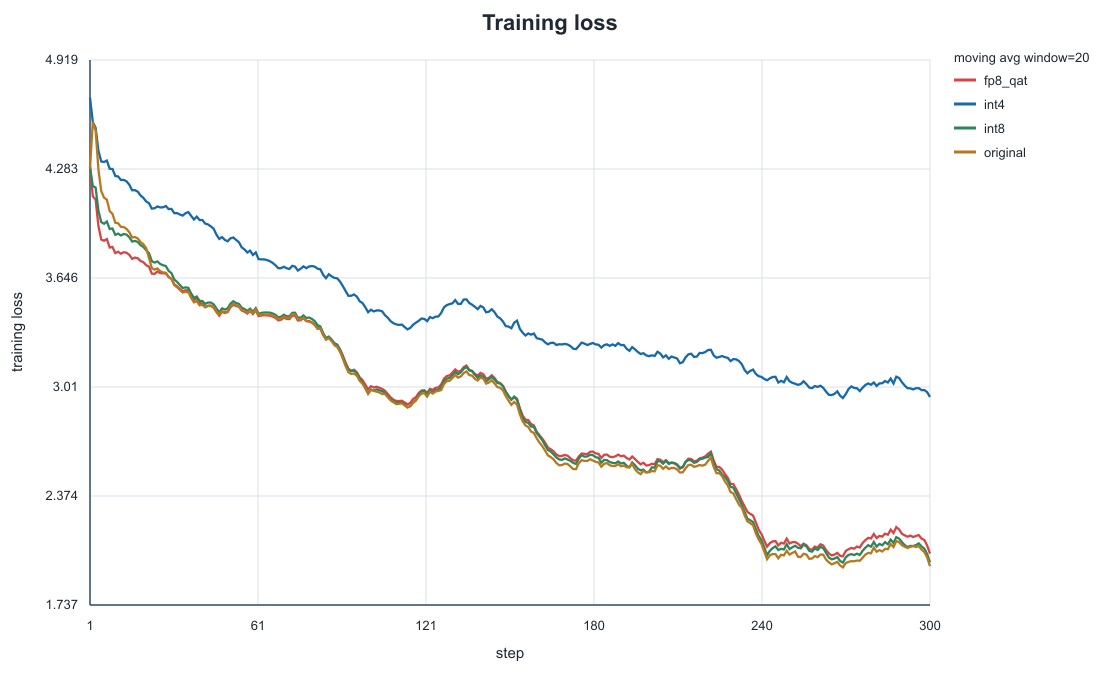
\includegraphics[width=\linewidth]{figures/fig1-weight-quant.png}
    \caption{FP8/INT8 weight QAT track the original run; INT4 trains but lags.}
    \label{fig:weight-precision}
  \end{subfigure}
  \hfill
  \begin{subfigure}{0.49\linewidth}
    \centering
    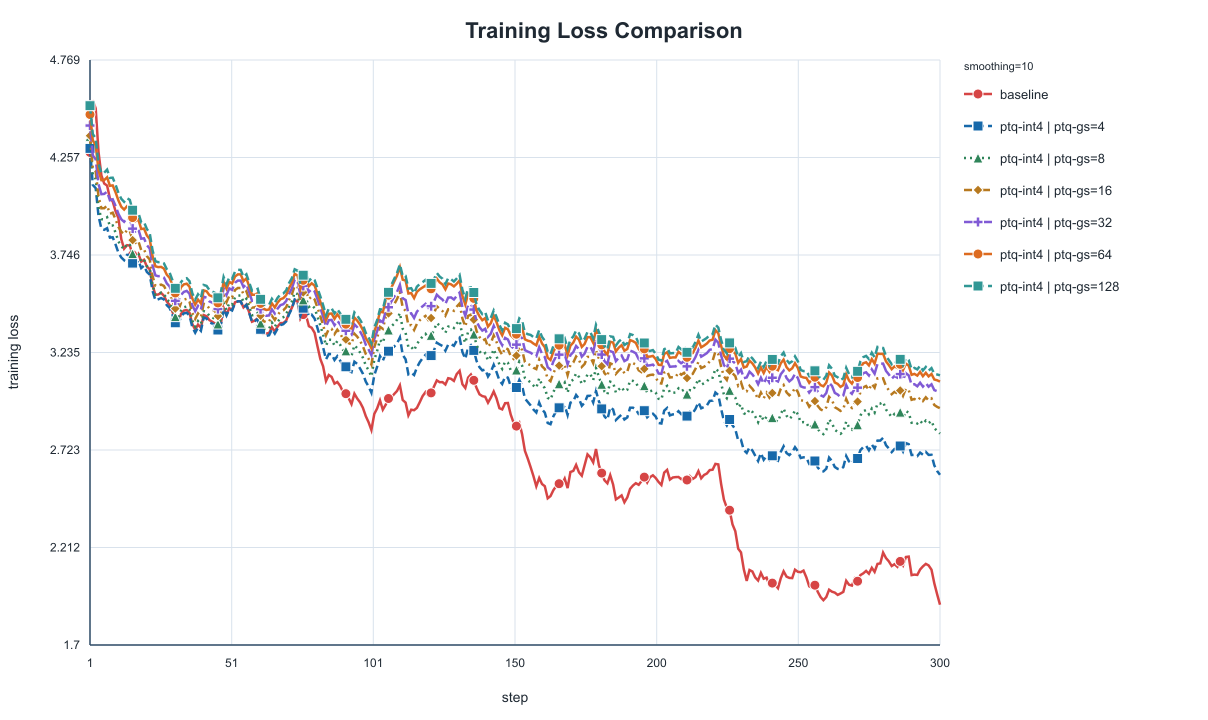
\includegraphics[width=\linewidth]{figures/fig2-int4-groups.png}
    \caption{Smaller INT4 groups preserve local dynamic range better.}
    \label{fig:int4-groups}
  \end{subfigure}
  \caption{Weight quantization results. The QAT infrastructure is stable for FP8 and INT8
  weights. INT4 requires finer group-wise scaling; group size 4 is the strongest tested
  INT4 setting.}
  \label{fig:weights}
\end{figure*}

Figure~\ref{fig:weights} compares the original model with \texttt{FP8}, \texttt{INT8}, and
\texttt{INT4} stored weights. \texttt{FP8} and \texttt{INT8} follow the original curve
closely, while \texttt{INT4} remains consistently higher. The group-size sweep explains the
gap: per-row or large-group scaling forces many unrelated values to share one scale, so
small weights are rounded away when a group contains larger values. Smaller groups preserve
local dynamic range and narrow the loss gap.

\subsection{Optimizer-State Quantization Works as a Memory Lever}

\begin{figure*}[htbp]
  \centering
  \begin{subfigure}{0.49\linewidth}
    \centering
    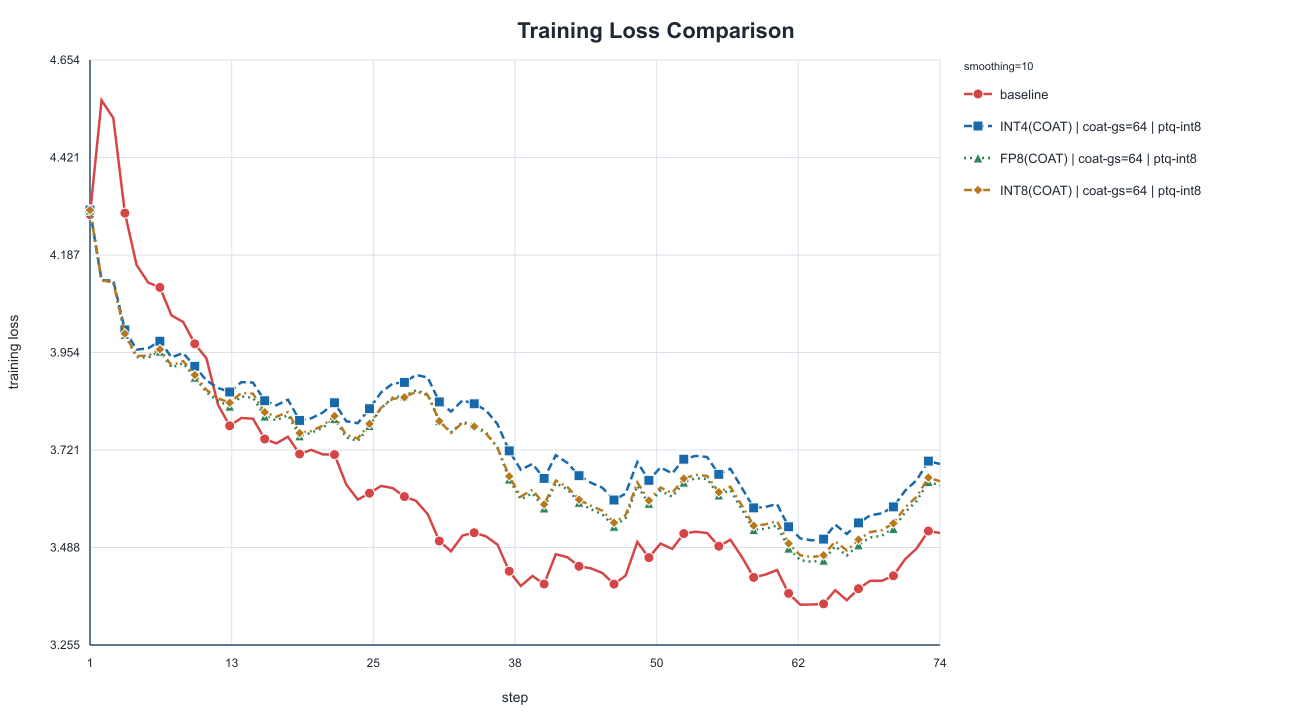
\includegraphics[width=\linewidth]{figures/fig3-optim-precision.png}
    \caption{FP8, INT8, and INT4 COAT-style moment storage all train in the short run.}
    \label{fig:optim-precision}
  \end{subfigure}
  \hfill
  \begin{subfigure}{0.49\linewidth}
    \centering
    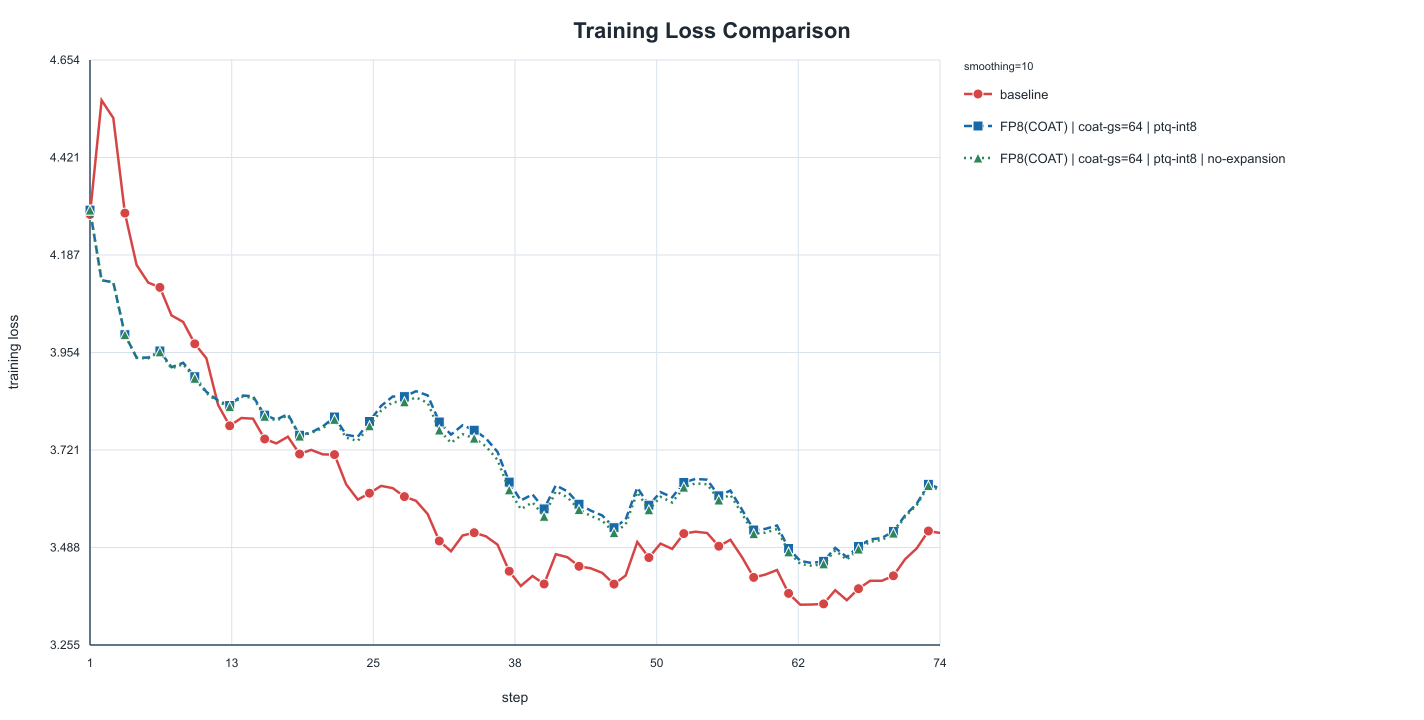
\includegraphics[width=\linewidth]{figures/fig4-dynamic-range.png}
    \caption{COAT expansion and no-expansion runs are similar for this distribution.}
    \label{fig:dre}
  \end{subfigure}
  \caption{Optimizer-state quantization results. Compressing AdamW moments is the largest
  persistent-state memory lever, and the low-precision moment formats do not immediately
  destabilize training.}
  \label{fig:optimizer}
\end{figure*}

Figure~\ref{fig:optimizer} shows that optimizer-state quantization is the main memory
contribution. AdamW's $m$ and $v$ buffers are normally \texttt{FP32}, so replacing them with
low-precision payloads plus per-group metadata gives a large persistent memory reduction.
The tested quantized optimizer paths remain close to each other, which suggests that
storing moments at low precision is less fragile than quantizing attention activations.
Dynamic range expansion does not visibly separate itself in this run because the observed
moment groups already have relatively narrow ranges, keeping the expansion factor close to
1.

\subsection{Activation Quantization Is the Failure Mode}

\begin{figure*}[htbp]
  \centering
  \begin{subfigure}{0.49\linewidth}
    \centering
    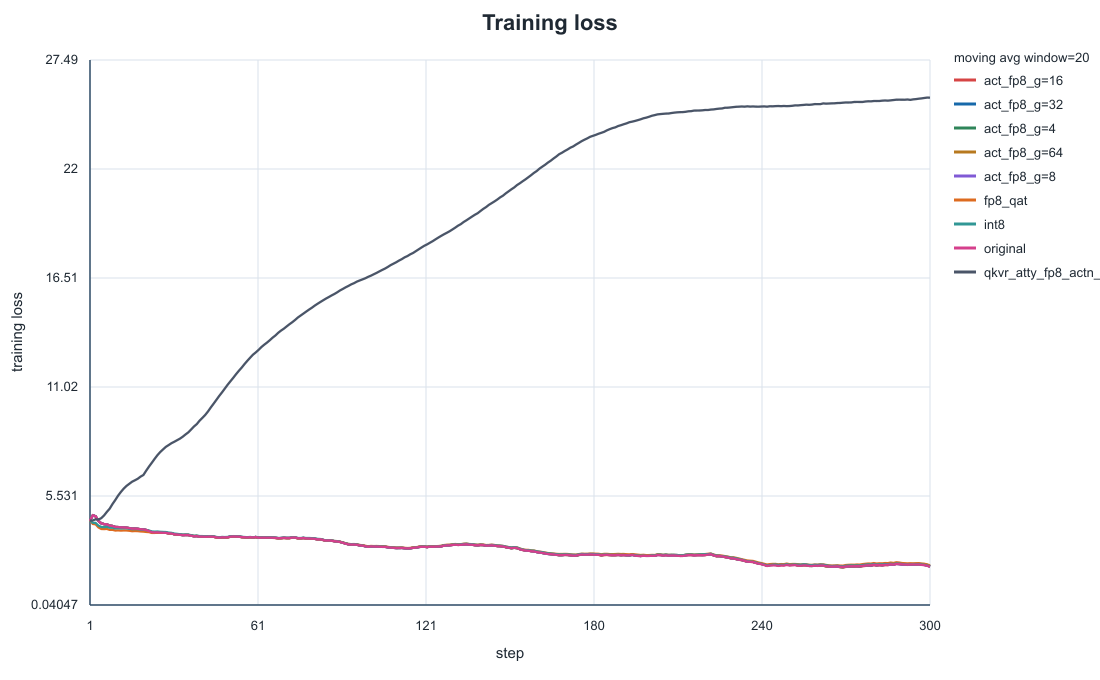
\includegraphics[width=\linewidth]{figures/fig5-activation-fail.png}
    \caption{Naively quantizing QKV projections and attention output diverges.}
    \label{fig:act-fail}
  \end{subfigure}
  \hfill
  \begin{subfigure}{0.49\linewidth}
    \centering
    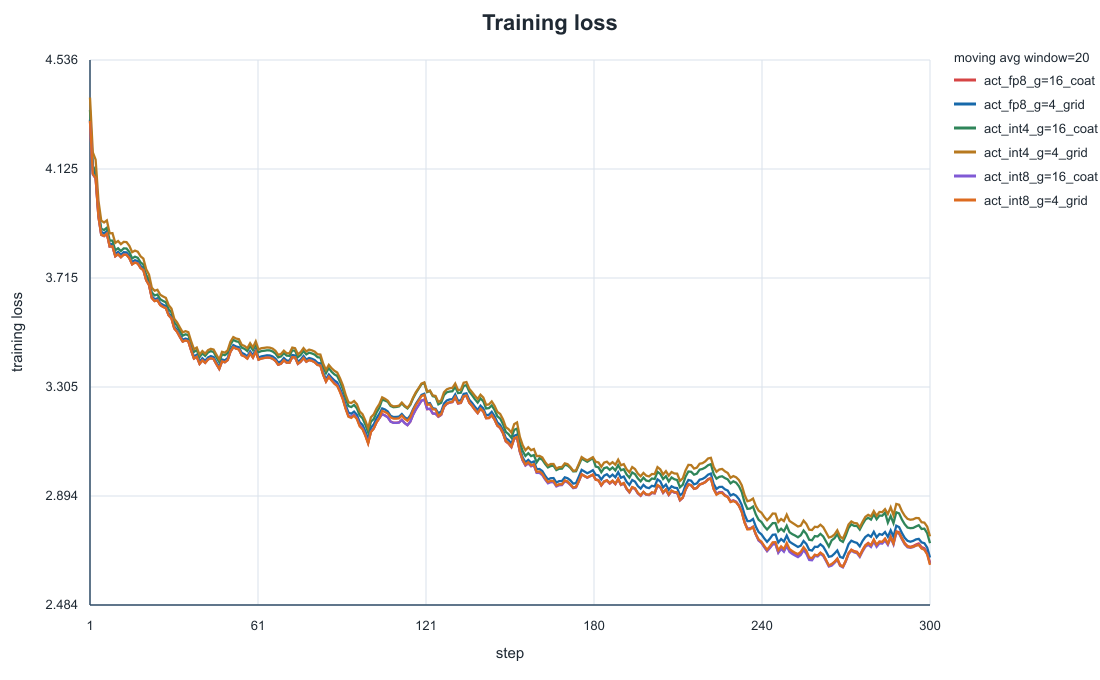
\includegraphics[width=\linewidth]{figures/fig6-activation-recovery.png}
    \caption{Row/COAT-style activation grouping restores stable training.}
    \label{fig:act-recover}
  \end{subfigure}
  \caption{Activation quantization results. The attention path is sensitive to activation
  quantization, but tensor-aware grouping recovers stable training behavior.}
  \label{fig:activation}
\end{figure*}

Figure~\ref{fig:activation} identifies the primary failure mode. A simple grid-style
activation quantizer is not sufficient for all tensors. The attention path is especially
sensitive because errors in Q/K/V projections affect attention scores, softmax
probabilities, and the backward signal. Row-wise grouping aligns better with Transformer
activation structure because values within a token row tend to share a more coherent
distribution than arbitrary $4\times4$ tiles. With that grouping, activation-quantized runs
remain in the same loss band as the other quantized runs.

\subsection{Memory Reduction}

\begin{figure}[htbp]
  \centering
  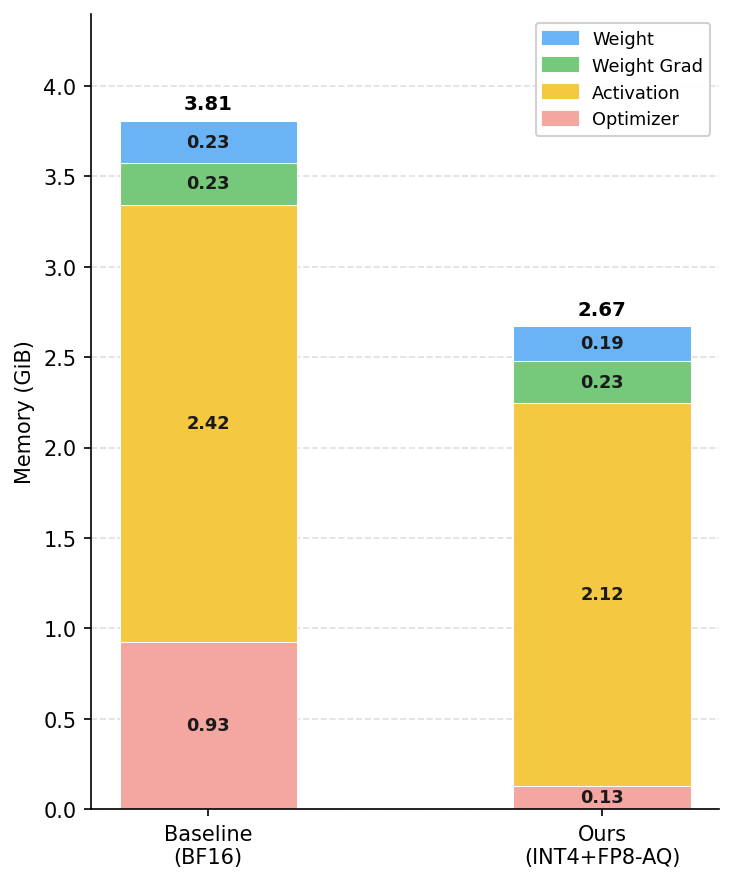
\includegraphics[width=0.42\linewidth]{figures/fig7-memory.png}
  \caption{Measured memory breakdown. The combined quantized configuration reduces total
  measured memory from 3.81 GiB to 2.67 GiB, a reduction of about 30\%.}
  \label{fig:memory}
\end{figure}

The memory result in Figure~\ref{fig:memory} is the main quantitative outcome. The baseline
BF16 run uses 3.81 GiB in the measured breakdown. The combined configuration, labeled
\texttt{INT4+FP8-AQ}, uses 2.67 GiB. This is a 1.14 GiB reduction, or approximately 30\%.
The optimizer block drops from 0.93 GiB to 0.13 GiB, confirming the central motivation for
optimizer-state quantization. Activation memory also falls from 2.42 GiB to 2.12 GiB, and
weight memory falls from 0.23 GiB to 0.19 GiB.

\begin{table*}[htbp]
  \centering
  \caption{Experimental conclusions.}
  \label{tab:summary}
  \begin{tabular}{lll}
    \toprule
    Component & Status & Evidence \\
    \midrule
    FP8/INT8 weights & Stable & 300-step loss curves track original closely \\
    INT4 weights & Works with tuning & Smaller groups reduce the loss gap \\
    COAT optimizer states & Promising & FP8, INT8, and INT4 moments train in short runs \\
    Activation quantization & Sensitive & Naive attention quantization diverges; row grouping recovers \\
    Memory & 30\% reduction & 3.81 GiB baseline to 2.67 GiB combined setup \\
    \bottomrule
  \end{tabular}
\end{table*}

\section{Conclusion}

This project implements a practical memory-efficient training path for GPT-2 in raw
C/CUDA. The cleanest completed piece is quantized weight storage for the four large
transformer projection matrices. These weights are stored as \texttt{INT8}, \texttt{FP8},
or grouped \texttt{INT4}, dequantized on demand for existing cuBLASLt matmuls, updated
through AdamW, and re-quantized after every step. That makes the implementation
functionally weight-only QAT even though the public flag is named \texttt{--ptq}.

The system also extends quantization to optimizer states. AdamW moments are stored in
\texttt{FP8}, \texttt{INT8}, or \texttt{INT4} with per-group scales and COAT-style dynamic
range expansion, while the actual optimizer math stays in \texttt{FP32}. This targets the
biggest persistent training-memory term after activations.

The final result is a coherent low-precision GPT-2 training pipeline. Low-precision weight
storage is stable for \texttt{FP8} and \texttt{INT8}, \texttt{INT4} becomes practical with
smaller groups, optimizer-state quantization preserves short-run training behavior, and
activation quantization becomes stable when grouping is aligned with Transformer tensor
structure. Combining these choices reduces measured memory from 3.81 GiB to 2.67 GiB while
preserving the decreasing training-loss trend. This demonstrates that a minimal C/CUDA
GPT-2 trainer can be extended beyond inference quantization into quantization-aware
training of weights, optimizer states, and activations.

\begin{thebibliography}{9}

\bibitem{jacob2017quantization}
B. Jacob, S. Kligys, B. Chen, M. Zhu, M. Tang, A. Howard, H. Adam, and
D. Kalenichenko.
\newblock Quantization and Training of Neural Networks for Efficient Integer-Arithmetic-Only Inference.
\newblock \emph{arXiv:1712.05877}, 2017.

\bibitem{dettmers2022llmint8}
T. Dettmers, M. Lewis, Y. Belkada, and L. Zettlemoyer.
\newblock LLM.int8(): 8-bit Matrix Multiplication for Transformers at Scale.
\newblock \emph{arXiv:2208.07339}, 2022.

\bibitem{xiao2022smoothquant}
G. Xiao, J. Lin, M. Seznec, H. Wu, J. Demouth, and S. Han.
\newblock SmoothQuant: Accurate and Efficient Post-Training Quantization for Large Language Models.
\newblock \emph{arXiv:2211.10438}, 2022.

\bibitem{xi2024coat}
H. Xi, H. Cai, L. Zhu, Y. Lu, K. Keutzer, J. Chen, and S. Han.
\newblock COAT: Compressing Optimizer States and Activations for Memory-Efficient FP8 Training.
\newblock \emph{arXiv:2410.19313}, 2024.

\bibitem{karpathyllmc}
A. Karpathy.
\newblock \texttt{llm.c}: LLM training in simple, raw C/CUDA.
\newblock \url{https://github.com/karpathy/llm.c}.

\end{thebibliography}

\end{document}
